\documentclass{oci}
\usepackage[utf8]{inputenc}
\usepackage{lipsum}
\usepackage{stackengine}

\title{Ajedrez}

\begin{document}
\begin{problemDescription}
  El ajedrez es un juego de tablero conocido por su dificultad.
  Los mejores jugadores del mundo destacan por su capacidad de anticiparse a todas las posibles jugadas.
  El juego tiene ya casi 1500 años, pero continúa siendo muy popular y en la actualidad siguen desarrollándose nuevas técnicas y estrategias.
  
  El ajedrez se juega entre dos personas sobre un tablero de $8\times 8$ casillas.
  Cada jugador tiene a su disposición un conjunto de piezas que debe mover estratégicamente para lograr vencer a su oponente.
  En cada turno un jugador debe mover una de sus piezas desde una casilla a otra.
  En el ajedrez, cada tipo de pieza tiene distintas reglas para poder moverse.
  En este problema solo nos interesa la forma en que puede moverse cada tipo de pieza sobre un tablero.
  
  Consideraremos el movimiento de 5 tipos de piezas: la torre, el alfil, la reina, el rey y el caballo.
  A continuación se describen las reglas de movimiento de cada pieza.
  Adicionalmente, la figura de más abajo muestra las posibles casillas en un tablero de $5\times 5$ a las que podría moverse cada pieza en un solo movimiento.
  \begin{itemize}
    \item \textbf{Torre:} La torre puede moverse en línea recta de forma horizontal o vertical cuantas casillas quiera en un movimiento.
    \item \textbf{Alfil:} El alfil puede moverse a lo largo de una diagonal cuantas casillas quiera en un movimiento.
    \item \textbf{Reina:} La reina es una combinación de la torre y el alfil, ya que puede moverse en diagonal, horizontal o verticalmente cuantas casillas quiera en un movimiento.
    \item \textbf{Rey:} El rey, al igual que la reina, puede moverse en cualquier dirección pero solo una casilla por movimiento.
    \item \textbf{Caballo:} El caballo es la pieza con el movimiento más complicado. Su movimiento es en forma de ``L'', es decir, siempre se mueve 2 casillas en una dirección (horizontal o vertical), y luego una casilla en la otra dirección.
  \end{itemize}
  
  \begin{center}
  \small
  \stackunder{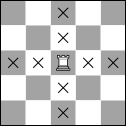
\includegraphics[scale=0.7]{rook.png}}{\bf Torre}
  \stackunder{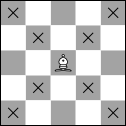
\includegraphics[scale=0.7]{bishop.png}}{\bf Alfil}
  \stackunder{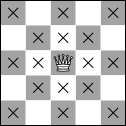
\includegraphics[scale=0.7]{queen.png}}{\bf Reina}
  \stackunder{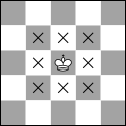
\includegraphics[scale=0.7]{king.png}}{\bf Rey}
  \stackunder{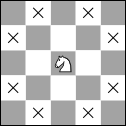
\includegraphics[scale=0.7]{knight.png}}{\bf Caballo}
  \end{center}
  
  Tu tarea consiste en crear un programa que determine la mínima cantidad de movimientos en los que es posible llevar una pieza desde una casilla a otra en un tablero de $100\times 100$
\end{problemDescription}

\begin{inputDescription}
  La entrada consiste en 3 líneas.
  
  La primera línea contiene un único entero $P$, que representa el tipo de pieza que se desea mover (torre=1, alfil=2, reina=3, rey=4, caballo=5).
  
  La segunda línea contiene dos enteros $X_{i}$ y $Y_{i}$, correspondientes a las coordenadas de la posición inicial de la pieza.
  El valor $X_{i}$ corresponde a la columna de la casilla en el tablero, mientras que $Y_{i}$ corresponde a la fila.
  Las columnas y filas del tablero son numeradas con con valores entre 0 y 99, de izquierda a derecha y de abajo hacia arriba.
  La columna de más a la izquierda corresponde a la columna 0 y la de más a la derecha a la columna 99.
  La fila de más abajo corresponde a la fila 0 y la de más arriba a la fila 99.
  
  La tercera línea de la entrada contiene dos enteros $X_{f}$ y $Y_{f}$ correspondientes a las coordenadas de la posición donde se quiere mover la pieza.
  
  Los valores de $X_i$, $Y_i$, $X_f$ y $X_f$ siempre serán mayores o iguales que 0 y menores o iguales que 99.
  Además $P$ siempre representará una pieza válida, es decir, $1 \le P \le 5$.
\end{inputDescription}

\begin{outputDescription}
  Tu programa debe imprimir una única línea con un entero: el número mínimo de movimientos en que es posible llevar la pieza desde la casilla inicial a la final.
  Si no es posible mover la pieza desde la casilla inicial a la final tu programa debe imprimir -1.
\end{outputDescription}

\begin{scoreDescription}
  \score{20} Se probarán varios casos solo con torres (P=1)
  \score{20} Se probarán varios casos solo con alfiles (P=2)
  \score{20} Se probarán varios casos solo con reinas (P=3)
  \score{20} Se probarán varios casos solo con reyes (P=4)
  \score{20} Se probarán varios casos solo con caballos (P=5)
\end{scoreDescription}

\begin{sampleDescription}
 \sampleIO{sample1}
 \sampleIO{sample2}
 \sampleIO{sample3}
 \sampleIO{sample4}
 \sampleIO{sample5}
 \sampleIO{sample6}
\end{sampleDescription}

\end{document}
